% Sandbox of the paper text_causal_latent.tex
\documentclass[12pt]{article}
\usepackage[utf8]{inputenc}
\usepackage[T1]{fontenc}
\usepackage{amsmath,amsfonts,amssymb}
\usepackage{graphicx}
\usepackage{a4wide}
\usepackage{xypic}

\newcommand{\T}{^{\mathsf{T}}}
\newcommand{\eL}{\mathcal{L}}

\title{Causal inference in latent space for time series and text data}
\author{IA pour la Science}
\date{30 january 2026}
\begin{document}
%+++++++++++++++++++++++++++++++++++++++++

%+++++++++++++++++++++++++++++++++++++++++

\maketitle
\section*{Introduction}
We construct a Bayesian causal-inference model for multivariate time series.
The goal is to identify a causal relationship between time series given the constructed model.
We suppose that the unknown dynamics generated the observable time series from the latent space.
Here we keep the model simple to expand it for
    1) multimodal time series and control problems,
    2) transformers and large models,
    3) continuous-time dynamical systems and Neural ODE.

\section{Autoregression model for linear dynamical system in latent space}
There given time series $\mathbf{x}_t$ as observations.
The time series are generated by a discrete-time dynamical system in the latent space~$\mathbf{z}_t$ with unknown dynamics:
\[ \mathbf{y}_{t+1} = f\bigl(\mathbf{z}_t, \mathbf{x}_t, \mathbf{y}_t\bigr)  + \boldsymbol{\zeta}_{t+1},\]

The time series are represented via \emph{delay embedding}.
The matrix of delay vectors for the scalar-valued series~$x_t$ is the Hankel matrix:

\iffalse
\[
\mathbf{W}
=
\begin{pmatrix}
w_{1,1} & w_{1,2} & \cdots & w_{1,K} \\
w_{2,1} & w_{2,2} & \cdots & w_{2,K} \\
\vdots  & \vdots  & \w_{\tau,\kappa} & \vdots  \\
w_{T,1} & w_{T,2} & \cdots & w_{T,K}
\end{pmatrix},
\qquad
w_{\tau,\kappa},\;
\tau=1,\dots,T,\;
\kappa=1,\dots,K
\]
\fi

\[\mathbf{X} = \begin{pmatrix}
x_{t-1} & x_{t-2} & \cdots & x_{t-(N+T}) \\
x_{t-2} & x_{t-3} & \cdots & x_{t-(N+T-1)} \\
\vdots & \vdots & x_{t-\tau} & \vdots \\
x_{t-N} & x_{t-(N-1)} & \cdots & x_{T}
\end{pmatrix},\] %\[\mathbf{X} = \begin{pmatrix} x(t_1) & x(t_2) & \cdots & x(t_{N-T}) \\ x(t_1 - \Delta t) & x(t_2 - \Delta t) & \cdots & x(t_{N-T} - \Delta t) \\ \vdots & \vdots & \ddots & \vdots \\ x(t_1 - (T-1)\Delta t) & x(t_2 - (T-1)\Delta t) & \cdots & x(t_{N-T} - (T-1)\Delta t) \end{pmatrix},\]
where $T\ni\{1,\dots,t\}$ is the sample size, $N$ is the original embedding dimension, and the time lag~$\Delta t = 1$.
A column of this matrix contains a point~$\mathbf{x}_t$ in the state space.
The sequence~$\{\mathbf{x}_t\}$ forms the phase trajectory~$\mathbf{X}$.
Call the \emph{embedding} the linear map $\mathbf{z}=\mathbf{U}\mathbf{x}$.
% TODO include an example with the phase trajectory


\section{Bayesian inferecence}
For the posterior distribution of the model parameters~$\mathbf{w}$ given the data~$\{\mathbf{x}, \mathbf{y}\}$, we have
\[
    p(\mathbf{w}|\mathbf{x}, \mathbf{y}) = \frac{p(\mathbf{y}|\mathbf{x}; \mathbf{w}) p(\mathbf{w}|\mathbf{x})}{p(\mathbf{y}|\mathbf{x})}.
\]
The likelihood function is defined as
\[p(\mathbf{y}|\mathbf{x}; \mathbf{w}) = \prod_{t=1}^T p(\mathbf{y}_t|\mathbf{x}_t; \mathbf{w}).\]
The error given the posterior distribution of the parameters is
\[
\eL(\mathbf{x}) = \frac{1}{2}(\mathbf{f}-\mathbf{y})\T \mathbf{B}^{-1}(\mathbf{f}-\mathbf{y}) +\frac{1}{2} (\mathbf{w} - \boldsymbol{\mu})\T \mathbf{A}^{-1}(\mathbf{w} - \boldsymbol{\mu}).
\]
Here we consider the matrix $\mathbf{B}=\beta I$ for the hypothesis that the variance~$\beta$ of the reconstruction error the same in the time segment $(1,\dots,T)$.
%\iffalse

\section{Technical details}
Put the backprop here and tell how to compute sequence of layers.

\iffalse
\section*{Backpropagation in a Fully Connected Neural Network}

\subsection*{Network Definition}

Consider a fully connected feedforward neural network with $L$ layers (excluding the input layer).
For layer $\ell = 1, \dots, L$:

\begin{itemize}
  \item Weight matrix: $\bm{W}^{(\ell)} \in \mathbb{R}^{n_\ell \times n_{\ell-1}}$
  \item Bias vector: $\bm{b}^{(\ell)} \in \mathbb{R}^{n_\ell}$
  \item Pre-activation: $\bm{z}^{(\ell)} \in \mathbb{R}^{n_\ell}$
  \item Activation: $\bm{a}^{(\ell)} \in \mathbb{R}^{n_\ell}$
\end{itemize}

The input is $\bm{a}^{(0)} = \bm{x}$.

\subsection*{Forward Propagation}

For $\ell = 1, \dots, L$:
\begin{align}
\bm{z}^{(\ell)} &= \bm{W}^{(\ell)} \bm{a}^{(\ell-1)} + \bm{b}^{(\ell)} \\
\bm{a}^{(\ell)} &= \sigma^{(\ell)}\!\left( \bm{z}^{(\ell)} \right)
\end{align}

where $\sigma^{(\ell)}(\cdot)$ is the activation function of layer $\ell$.

Let the network output be $\hat{\bm{y}} = \bm{a}^{(L)}$.

\subsection*{Loss Function}

Let $\mathcal{L}(\hat{\bm{y}}, \bm{y})$ be a scalar loss function comparing prediction $\hat{\bm{y}}$
with target $\bm{y}$.

\subsection*{Backpropagation}

Define the error signal (gradient of the loss with respect to pre-activation):
\[
\bm{\delta}^{(\ell)} \equiv \frac{\partial \mathcal{L}}{\partial \bm{z}^{(\ell)}}
\]

\subsubsection*{Output Layer}

Using the chain rule:
\begin{align}
\bm{\delta}^{(L)}
&= \frac{\partial \mathcal{L}}{\partial \bm{a}^{(L)}}
\odot \sigma'^{(L)}\!\left(\bm{z}^{(L)}\right)
\end{align}

where $\odot$ denotes element-wise multiplication.

\subsubsection*{Hidden Layers}

For $\ell = L-1, \dots, 1$:
\begin{align}
\bm{\delta}^{(\ell)}
&= \left( \bm{W}^{(\ell+1)} \right)^{\!\top} \bm{\delta}^{(\ell+1)}
\odot \sigma'^{(\ell)}\!\left(\bm{z}^{(\ell)}\right)
\end{align}

\subsection*{Gradients with Respect to Parameters}

Using the definition of $\bm{\delta}^{(\ell)}$:

\begin{align}
\frac{\partial \mathcal{L}}{\partial \bm{W}^{(\ell)}}
&= \bm{\delta}^{(\ell)} \left( \bm{a}^{(\ell-1)} \right)^{\!\top} \\
\frac{\partial \mathcal{L}}{\partial \bm{b}^{(\ell)}}
&= \bm{\delta}^{(\ell)}
\end{align}

\subsection*{Summary (Vectorized Form)}

For each layer $\ell$:
\[
\boxed{
\begin{aligned}
\bm{z}^{(\ell)} &= \bm{W}^{(\ell)} \bm{a}^{(\ell-1)} + \bm{b}^{(\ell)} \\
\bm{a}^{(\ell)} &= \sigma^{(\ell)}(\bm{z}^{(\ell)}) \\
\bm{\delta}^{(\ell)} &=
\begin{cases}
\dfrac{\partial \mathcal{L}}{\partial \bm{a}^{(L)}} \odot \sigma'^{(L)}(\bm{z}^{(L)}), & \ell = L \\
\left( \bm{W}^{(\ell+1)} \right)^{\!\top} \bm{\delta}^{(\ell+1)}
\odot \sigma'^{(\ell)}(\bm{z}^{(\ell)}), & \ell < L
\end{cases} \\
\frac{\partial \mathcal{L}}{\partial \bm{W}^{(\ell)}} &= \bm{\delta}^{(\ell)} (\bm{a}^{(\ell-1)})^\top \\
\frac{\partial \mathcal{L}}{\partial \bm{b}^{(\ell)}} &= \bm{\delta}^{(\ell)}
\end{aligned}
}
\]
\fi

\subsection{Neural ODE}
Put the idea how to compute CI for continuous time dynamical system.

Set the forecasting model
\[f: \mathbf{x}\to \mathbf{y}\]
as a linear operator.
Introduce the singular value decomposition $f=U\Lambda V^\mathsf{T}$:
\begin{equation*}
    \xymatrix{
        \mathbf{x} \ar "1,3"^{f} \ar "2,2"_{\mathbf{U}} & ~  & \mathbf{y} \\% \ar "2,2"_{\mathbf{V^\mathsf{T}}}  \\
        ~ & \mathbf{z} \ar "1,3"_{\mathbf{V}^\mathsf{T}} & ~ \\
    ~ & t \ar "2,2"^{p(\mathbf{z}|t)} & ~
    }
\end{equation*}

The system dynamics is represented by the generative model~$p(\mathbf{z})$ that approximates the embedding in the latent space with the support $t$.

Treat this superposition as a decoder and a encoder, where the linear operators $\mathbf{U}$ and $\mathbf{V}$ are the orthogonal and $\Lambda$ is diagonal with positive elements.
Each row of the matrix
\[
\mathbf{U}\mathbf{x} =
    \begin{pmatrix}
        \mathbf{u}_1 \\ \mathbf{u}_2 \\ \vdots \\ \mathbf{u}_k
    \end{pmatrix}^\mathsf{T} \mathbf{x}
\]
 produces an element of a vector~$\mathbf{z}$ in the latent space by the dot product
\[z_i = \mathbf{u}_i^\mathsf{T} \mathbf{x}.\]

\subsection{The probabilistic view}
Let the prior distribution of a vector~$\mathbf{u} \sim \mathcal{N}(\mathbf{u}, \mathbf{A})$.
Its parameters are estimated as empirical distribution from the data.
As a criteion of the causal relationship between the elements of the model,
we use the Kullback-Leibler divergence between the distributions of the parameters given the intervention~$do(\mathbf{x})$:
\[\text{KL}\bigl(p(\mathbf{w}|do(X)\,||\,p(\mathbf{w}|do(X=\mathbf{x}_0)\bigr),\]
where~$\mathbf{w} = \{\mathbf{U}\}$ is the set of the model parameters.

For several layers of a neural network
\[
    f = \boldsymbol{\sigma}_L \circ \mathbf{W}_L \circ \boldsymbol{\sigma}_{L-1} \circ \mathbf{W}_{L-1} \circ \cdots \circ \boldsymbol{\sigma}_1 \circ \mathbf{W}_1 \mathbf{x},
\]

\section{The intervention algorithm}
\begin{enumerate}
    \item One step of back-prop in one layer.
    \item Compute the covariance of the parameters (note the relation between Cov, Hessian and Fisher matrices).
    \item Select a node~$X$ to make an intervention.
    \item Make an intervention $do(X=\mathbf{x}_0)$ for a given node.
    \item Compute the KL divergence between the distributions of the parameters with and without intervention.
    \item Remove the intervention and go to step~1 until all nodes are processed.
    \item The causal graph is constructed as a directed graph with edges weighted by the KL divergences.
\end{enumerate}

For a linear operator~$W^T$, elimination of an edge from a node~$X$
is equivalent to zeroing the corresponding item~$w_{ij}$.
The node~$X$ corresponds to a column in~$W$.

Since the item~$w$ acts both as a parameter and as a random variable, the following statement holds:

\begin{table}[h]
    \caption{The action for a node based on the variance of the parameter~$w$.}
    \begin{tabular}{|l|l|l|l|}
        \hline
        \bf{Expectation} & \bf{Variance} & \bf{Statement} & \bf{Action} \\ \hline \hline
        0       & tends to 0        & Sure that there is no impact  & Remove the node\\
        0       & not tends to 0    & Uncertain about the impact    & Research to remove\\
        not 0   & tends to 0        & Sure that there is an impact  & Assert the node\\
        not 0   & not tends to 0    & The impact must be specified  & Research to assert\\
        any     & large values      & Sure that there is no impact  & Remove the node\\
        \hline
    \end{tabular}
\end{table}

%+++++++++++++++++++++++++++++++++++++++++
%\fi
%+++++++++++++++++++++++++++++++++++++++++

% TODO Insert an algorithm how to sample the \emph{empirical} parameter distribution (estimate the expectation and variance).



\section{Consequent causal inference}
Results of the computational experiment: the norm of the gradient
$\|\frac{\partial \eL}{\partial W}\|_2$
of the layer (l) causes the norm of the gradient in the previous layer $l-1$
\[
    \Big\|\frac{\partial \eL}{\partial W^{(l)}}\Big\|_2 \leadsto \Big\|\frac{\partial \eL}{\partial W^{(l-1)}}\Big\|_2.
\]
As well as the error on the training set causes the error on the validation set,
\[
    L_\text{train} \leadsto L_\text{validation}.
\]
This holds for different optimization sessions.


\section{Do(X) intervention policy}
For regression or one-class classification, $do(X = x)$ is considered with values of $x$ that lie outside the distribution of the time series at time $t$.
For two-class classification, $do(X = x)$ is considered with values of $x$ equal to the expectation of the opposite class.

What happens after the intervention?
Until the forecasting and reconstruction error remains the same:
\[
    \eL\bigl(p(\mathbf{y}|\mathbf{x}; \mathbf{w})\bigr) = \text{const},
\]

When the error increases, The model parameters change.

Until the end of the short-term forecast horizon.

From one of sides, either X or Z, we start the intervention.
Start with the parameter of maximum variance of reconstruction error
Then, move to the parameters with lower variance.
Estimate the KL divergence of maximum posterior after each intervention.
Analyse the expectation and the variance of the parameters.
Eliminate the parameters with the highest KL divergence.
Keep the parameters with the lowest KL divergence.
Store them in the graph of causality.

%-----------------------------------------
Compare two graphs: direct and reverse.
%-----------------------------------------




\section{Relations between the Hessain, Fisher, and Covariance matrices of the parameters}
The Hessian matrix of the loss function~$\eL$ is defined as
\[\mathbf{H} = \frac{\partial^2 \eL}{\partial \mathbf
{w} \partial \mathbf{w}^\mathsf{T}}.\]
Using the log-likelihood function, we have
\[
 %   \mathbf{H} = \mathbb{E}\Bigg[{\frac{\partial^2 \log p(\mathbf{y}|\mathbf{x}; \mathbf{w})}{\partial \mathbf{w} \partial \mathbf{w}^\math{T}}}\Bigg].
\]
Using the posterior of the parameters, we have
\[
%    \mathbf{H} = \mathbb{E}\Bigg[{\frac{\partial^2 \log p(\mathbf{w}|\mathbf{x}, \mathbf{y})}{\partial \mathbf{w} \partial \mathbf{w}^\math{T}}}\Bigg].
\]

The Fisher information matrix is defined as
\[\mathbf{F} = \mathbb{E}\Bigg[\Big(\frac
{\partial \log p(\mathbf{y}|\mathbf{x}; \mathbf{w})}{\partial \mathbf{w}}\Big)\Big(\frac{\partial \log p(\mathbf{y}|\mathbf{x}; \mathbf{w})}{\partial \mathbf{w}}\Big)^\mathsf{T}\Bigg].\]
Under certain regularity conditions, the following relation holds:
\[\mathbf{H} = -\mathbf{F}.\]
The covariance matrix of the parameters~$\mathbf{w}$ is defined as
\[\mathbf{C} = \mathbb{E}\Big[(\mathbf{w} - \mathbb{E}[\mathbf{w}])(\mathbf{w} - \mathbb{E}[\mathbf{w}])^\mathsf{T}\Big].\]
Under certain assumptions, the following relation holds:
\[\mathbf{C} = \mathbf{F}^{-1}.\]
Thus, the Hessian, Fisher, and covariance matrices are interrelated and provide insights into the salience of the model parameters.




\section{Computational experiment}
For control problem we investigate a driven pendulum problem.
A pendulum of a given length has its own period of oscillation.
Driven by an external force a pendulum had forced oscillation.
These two oscillations are simple and independent.
They superposition are observed.
A change in the frequency of the driving force disturbs the superposition.
The goal is to identify the causal relationship between the driving force and the normal mode of the pendulum oscillations.

\newpage
\section{Appendix: Miscellaneous}

Todo: Put plate notations for the bayesian model structure~$\Gamma$ in the slides (on monday).
Introduce the bayesian structure of model~$\Gamma$ and associate it with the causal graph~$G$.
(The distribution of$\Gamma$ could be coincided with the weights of the edges in~$G$.)
The weights of the arrows in the causation model means the posterior model structure~$\Gamma$.

In the section 1: construct the manifold from the set of samples $\{\mathbf{z}\}$.
Then control this manifold and the variables~$do(Z=\mathbf{z})$ to infer the forecasting model~$f$.
Weight change and distribution as new data.
Change parameters of the generative model~$p(\mathbf{z})$ and observe changes in the forecast.
Use Variational Autoencoder instead of Normalising Flows.
It simplifies the generative model.

Discussion in January.
Check the error:
Infer another time series.
It changes parameter, but does not changes the forecast.
The error can stay the same.


Insert into section 2: Intervention in neuron weights versus intervention in the input data: proof of pros and cons.

We apply do()  the sin to reconstruct the trajectory. We know the sin since we know the trajectory could be reduced to dim=2.

Review: Hypothesis of \emph{mélange} by M.S.~Pinsker, or Ergodic Theory by Y.G.~Sinai is exactly the Causal Inference.
% Remark on Review: The problem of CI for LLM is all works I found are technical. It requires working infrastructure (code, computational resources). The papers on CI for LLM came through are technical, of specific purpose, mainty on linguestics, not data analysis and equire specific progrmming setup. The most interesting starts for spatial time series.

Afterlife: When a Neural Network is a solution of the differential equation?
Use the Neural ODE to test Causality in the mathematical models.

Domain transfer by causality graph: same model different datasets

% CCA. Use the main purpose of CI to show that the dynamic system is the cause of the observed signals. We investigate state models of two different sets of observations: source and target.

\section{Appendix: Control problem and Canonical Correlation Analysis}
\begin{equation*}
    \xymatrix{
        \mathbf{X} \ar "1,3"^{F} \ar "2,2" ^{\mathbf{U}} & ~  & \mathbf{Y} \ar "2,2"_{\mathbf{V}}  \\
        ~ & \mathbf{P},\mathbf{Q}  & ~ \\
        ~ & t \ar "2,2"^{p(\mathbf{z})} & ~
    }
\end{equation*}

\section{Appendix: continuous time dynamical system and delay embedding}
For the continuous-time dynamical system, the state vector~$\mathbf{z}(t)$ evolves according to the differential equation
\[
    \frac{d\mathbf{z}(t)}{dt} = f\bigl(\mathbf{z}(t), \mathbf{x}(t), \mathbf{y}(t)\bigr)  + \boldsymbol{\varepsilon}(t),
\]
and the observed time series are generated from the state vector via the observation functions:
\[
    \mathbf{x}(t) = h_x\bigl(\mathbf{z}(t)\bigr) + \boldsymbol{\xi}_x(t), \quad
    \mathbf{y}(t) = h_y\bigl(\mathbf{z}(t)\bigr) + \boldsymbol{\xi}_y(t),
\]
where $\boldsymbol{\varepsilon}(t)$, $\boldsymbol{\xi}_x(t)$, and $\boldsymbol{\xi}_y(t)$ are noise terms.

The matrix of delay vectors for the scalar-valued series~$x_t$ is the Hankel matrix:
 \[
     \mathbf{X} = \begin{pmatrix} x(t_1) & x(t_2) & \cdots & x(t_{N-T}) \\ x(t_1 - \Delta t) & x(t_2 - \Delta t) & \cdots & x(t_{N-T} - \Delta t) \\ \vdots & \vdots & \ddots & \vdots \\ x(t_1 - (T-1)\Delta t) & x(t_2 - (T-1)\Delta t) & \cdots & x(t_{N-T} - (T-1)\Delta t) \end{pmatrix},
 \]
where $T$ is the length of the time series sample, $t\in(1,T)$.
The time lag is~$\Delta t$ and~$N$ is the embedding dimension.

The continuous-time forecasting model is a convolution of two functions: the input signal $x(t)$ and the kernel $K(t)$ that represents the system dynamics.
Thus, the output signal $y(t)$ can be expressed
in the kernel terms:
\[
y(t) = \int_{t-T}^{t} K(t - \tau) x(\tau) d\tau + \varepsilon(t).
\]
The vector form of this equation is:
\[
\mathbf{y}_t - \boldsymbol{\varepsilon}_t = \mathbf{K}^\mathsf{T} \mathbf{x}_t,
\]

\end{document}
\section{Convergent Cross-Mapping}

\section{Multivariate Causal Models}\label{sec:multivariate-causal-models}
Feature selection for the optimal latent space require the following assumptions:
\begin{enumerate}
    \item The system state is reconstructable for both observable sets.
    \item An error of reconstruction in each set has gaussian distribution.
    \item A non-empty causal dependency between the source and the target.
    \item This dependency comprises only the reconstructed components.
    \item It is linear in the latent space.
\end{enumerate}
Let the dependency be a linear map $A$ between the latent spaces of the source and the target.
Then, the problem of feature selection can be formulated as the following optimization problem:
\begin{equation}
\min_{S_x, S_y} \| Z_y - A Z_x \|_F^2 + \lambda_x \| S_x \|_1 + \lambda_y \| S_y \|_1,
\end{equation}
where $Z_x$ and $Z_y$ are the matrices of the selected features from the source and the target, respectively; $S_x$ and $S_y$ are the binary selection vectors; $\lambda_x$ and $\lambda_y$ are the regularization parameters; and $\|\cdot\|_F$ and $\|\cdot\|_1$ are the Frobenius and L1 norms, respectively.


#4. Variant 2 we need alignment with
#5. There is a basis in both spaces and there is a dependency as a
#6. bipartite graph
#7. triangular graph





Short description of the projects, 1--3 sentences.
\begin{enumerate}[1)]
\item \emph{The impact} is; what the project changes
\item \emph{The consistency} or reliability is; where is the science, proofs, and analysis in your project
\item \emph{The novelty} is; how the proposed solution differs from the alternatives
\item \emph{My contribution} is; put where your personal effort go
\item \emph{The project focuses} on; put the main message you defend
\end{enumerate}


\section{Resume}
The project \emph{Title} has the highest priority since, due to; put a brief motivation here.



\beamertemplatenavigationsymbolsempty
\documentclass{beamer}
\setbeamertemplate{footline}[page number]

\title{Causal inference for text data \\via convergent cross-mapping}
\author{IA pour la Science}
\date{December $12^\text{th}$, 2025}

\begin{document}
\begin{frame}
  \titlepage
\end{frame}
%=============================================
\begin{frame}{Causal inference for text data}

\begin{block}{The goal of research}
Propose the Bayesian causal inference in terms of generative modeling for text data.
\end{block}

\begin{block}{The focus}
Represent the text data as multivariate time series and use Convergent Cross-Mapping for Causal Inference. 
\end{block}

\begin{enumerate}
\item Reformulate the control problem as the $|\text{do}(X)$ intervention for dynamical systems.
\item Prepare the model selection pipeline with domain localization and dimensionality reduction.
\item  Generalise the CCM to Canonical Correlation Analysis and Attention.
\item Conduct a computational experiment on d-variate time series, including text and video.
\end{enumerate}
\end{frame}
%=============================================
\begin{frame}{Convergent Cross Mapping}

\begin{itemize}
    \item We observe a pair of dynamical systems $X$ and $Y$, whose true behavior is described by the manifolds $W_x$ and $W_y$ in their corresponding phase spaces.
    We can only infer information about these manifolds from their projections $M_x$ and $M_y$ onto the observed values of the time series $\{x_t\}_{t=1}^T$ and $\{y_t\}_{t=1}^T$ corresponding to these systems.
    
    \item \textbf{Cross Mapping}. From the phase trajectory of one system, $M_x$, we can predict the values of the second system: $y_t \simeq \hat{y}_t|M_x$. Similarly, we can construct predictions $\hat{x}_t|M_y$. The accuracy of these predictions indicates whether a causal relationship exists between the systems.
    
    \item \textbf{Convergence}. If such a relationship exists, the prediction quality should improve as the considered time interval $T$ increases.
\end{itemize}
\end{frame}
%=============================================
\begin{frame}{Convergent Cross Mapping Algorithm (1)}
\begin{enumerate}
    \item There given two time series $\{x_1, x_2, ..., x_T\}$ and $\{y_1, y_2, ..., y_T\}$ of length $T$.
    \item For the series $\{x_t\}_{t=1}^T$, construct history vectors of dimension $E$ with time lag $\tau$:
    $$ \mathbf{x}_t = \begin{pmatrix}
        x_t, & x_{t - \tau}, & x_{t - 2\tau}, & \dots, & x_{t - (E-1)\tau}
    \end{pmatrix}.$$
    \item In the \emph{phase} space $\mathbb{R}^E$, these history vectors form the \emph{phase trajectory} of the system:
   $$M_x = \{\mathbf{x}_t \ | \ t = 1 + (E - 1)\tau, ..., T \}.$$
    \item[4.] One has to build a prediction for the value $y_t$. To do this, find the $E + 1$ vectors from $M_x$ that are closest to $\mathbf{x}_t$ (in terms of, for example, the standard metric $d$ in $\mathbb{R}^n$). Sort their time indices $t_1, ..., t_{E+1}$ from the nearest to the farthest points
    $$ d_i = d(\mathbf{x}_t, \mathbf{x}_{t_i}), \quad d_1 < d_2 < ... < d_{E + 1}.$$
\end{enumerate}
\end{frame}

%=============================================
\begin{frame}{Convergent Cross Mapping Algorithm (2)}

\begin{enumerate}
    \item[5.] The estimate of the value $y_t$ is then constructed as a weighted sum of the series values at times $t_1, ..., t_{E+1}$:
    $$ \hat{y}_t|M_x = \sum_{i=1}^{E+1} \omega_i y(t_i),$$
    $$ \omega_i = \frac{u_i}{\displaystyle \sum_{j=1}^{E + 1}u_j}, \qquad 
       u_i = \text{exp}\Big(-\frac{d_i}{d_1}\Big), \qquad i = 1, ..., E+1.$$
    \item[6.] To assess the existence of dependence between the time series $\{x_t\}_{t=1}^T$ and $\{y_t\}_{t=1}^T$,   compute the Pearson correlation coefficient:
    $$ C_{yx} = \Bigg[\rho \Big( y, \hat{y}|M_x \Big) \Bigg]^2.$$
\end{enumerate}

\end{frame}
%=============================================
\begin{frame}{State space reconstruction}
\begin{itemize}
    \item Takens' theorem use delay vectors to reconstruct the internal structure of a dynamical system.
    \item When the condition $m \geq 2d + 1$ is satisfied, where $d$ is the embedding dimension, it becomes possible to reconstruct the system’s state space.
    \item In particular, the conclusions of Takens' theorem are used in CCM. The CCM algorithm is analogous to a statistical test and evaluates the causal relationship between two time series.
\end{itemize}
\end{frame}
%=============================================
\begin{frame}{Questions to discuss}
\begin{enumerate}
\item List machine learning problems with text data to illustrate cases of Causal Inference.
\item List cases where the text data are represented as time series.
\item List datasets for the experiment \\
~~~~~1) time series to illustrate, \\
~~~~~2) text data to test.
\end{enumerate}
\end{frame}

%=============================================
\begin{frame}{Appendix: text data as time series, illustration (1)}

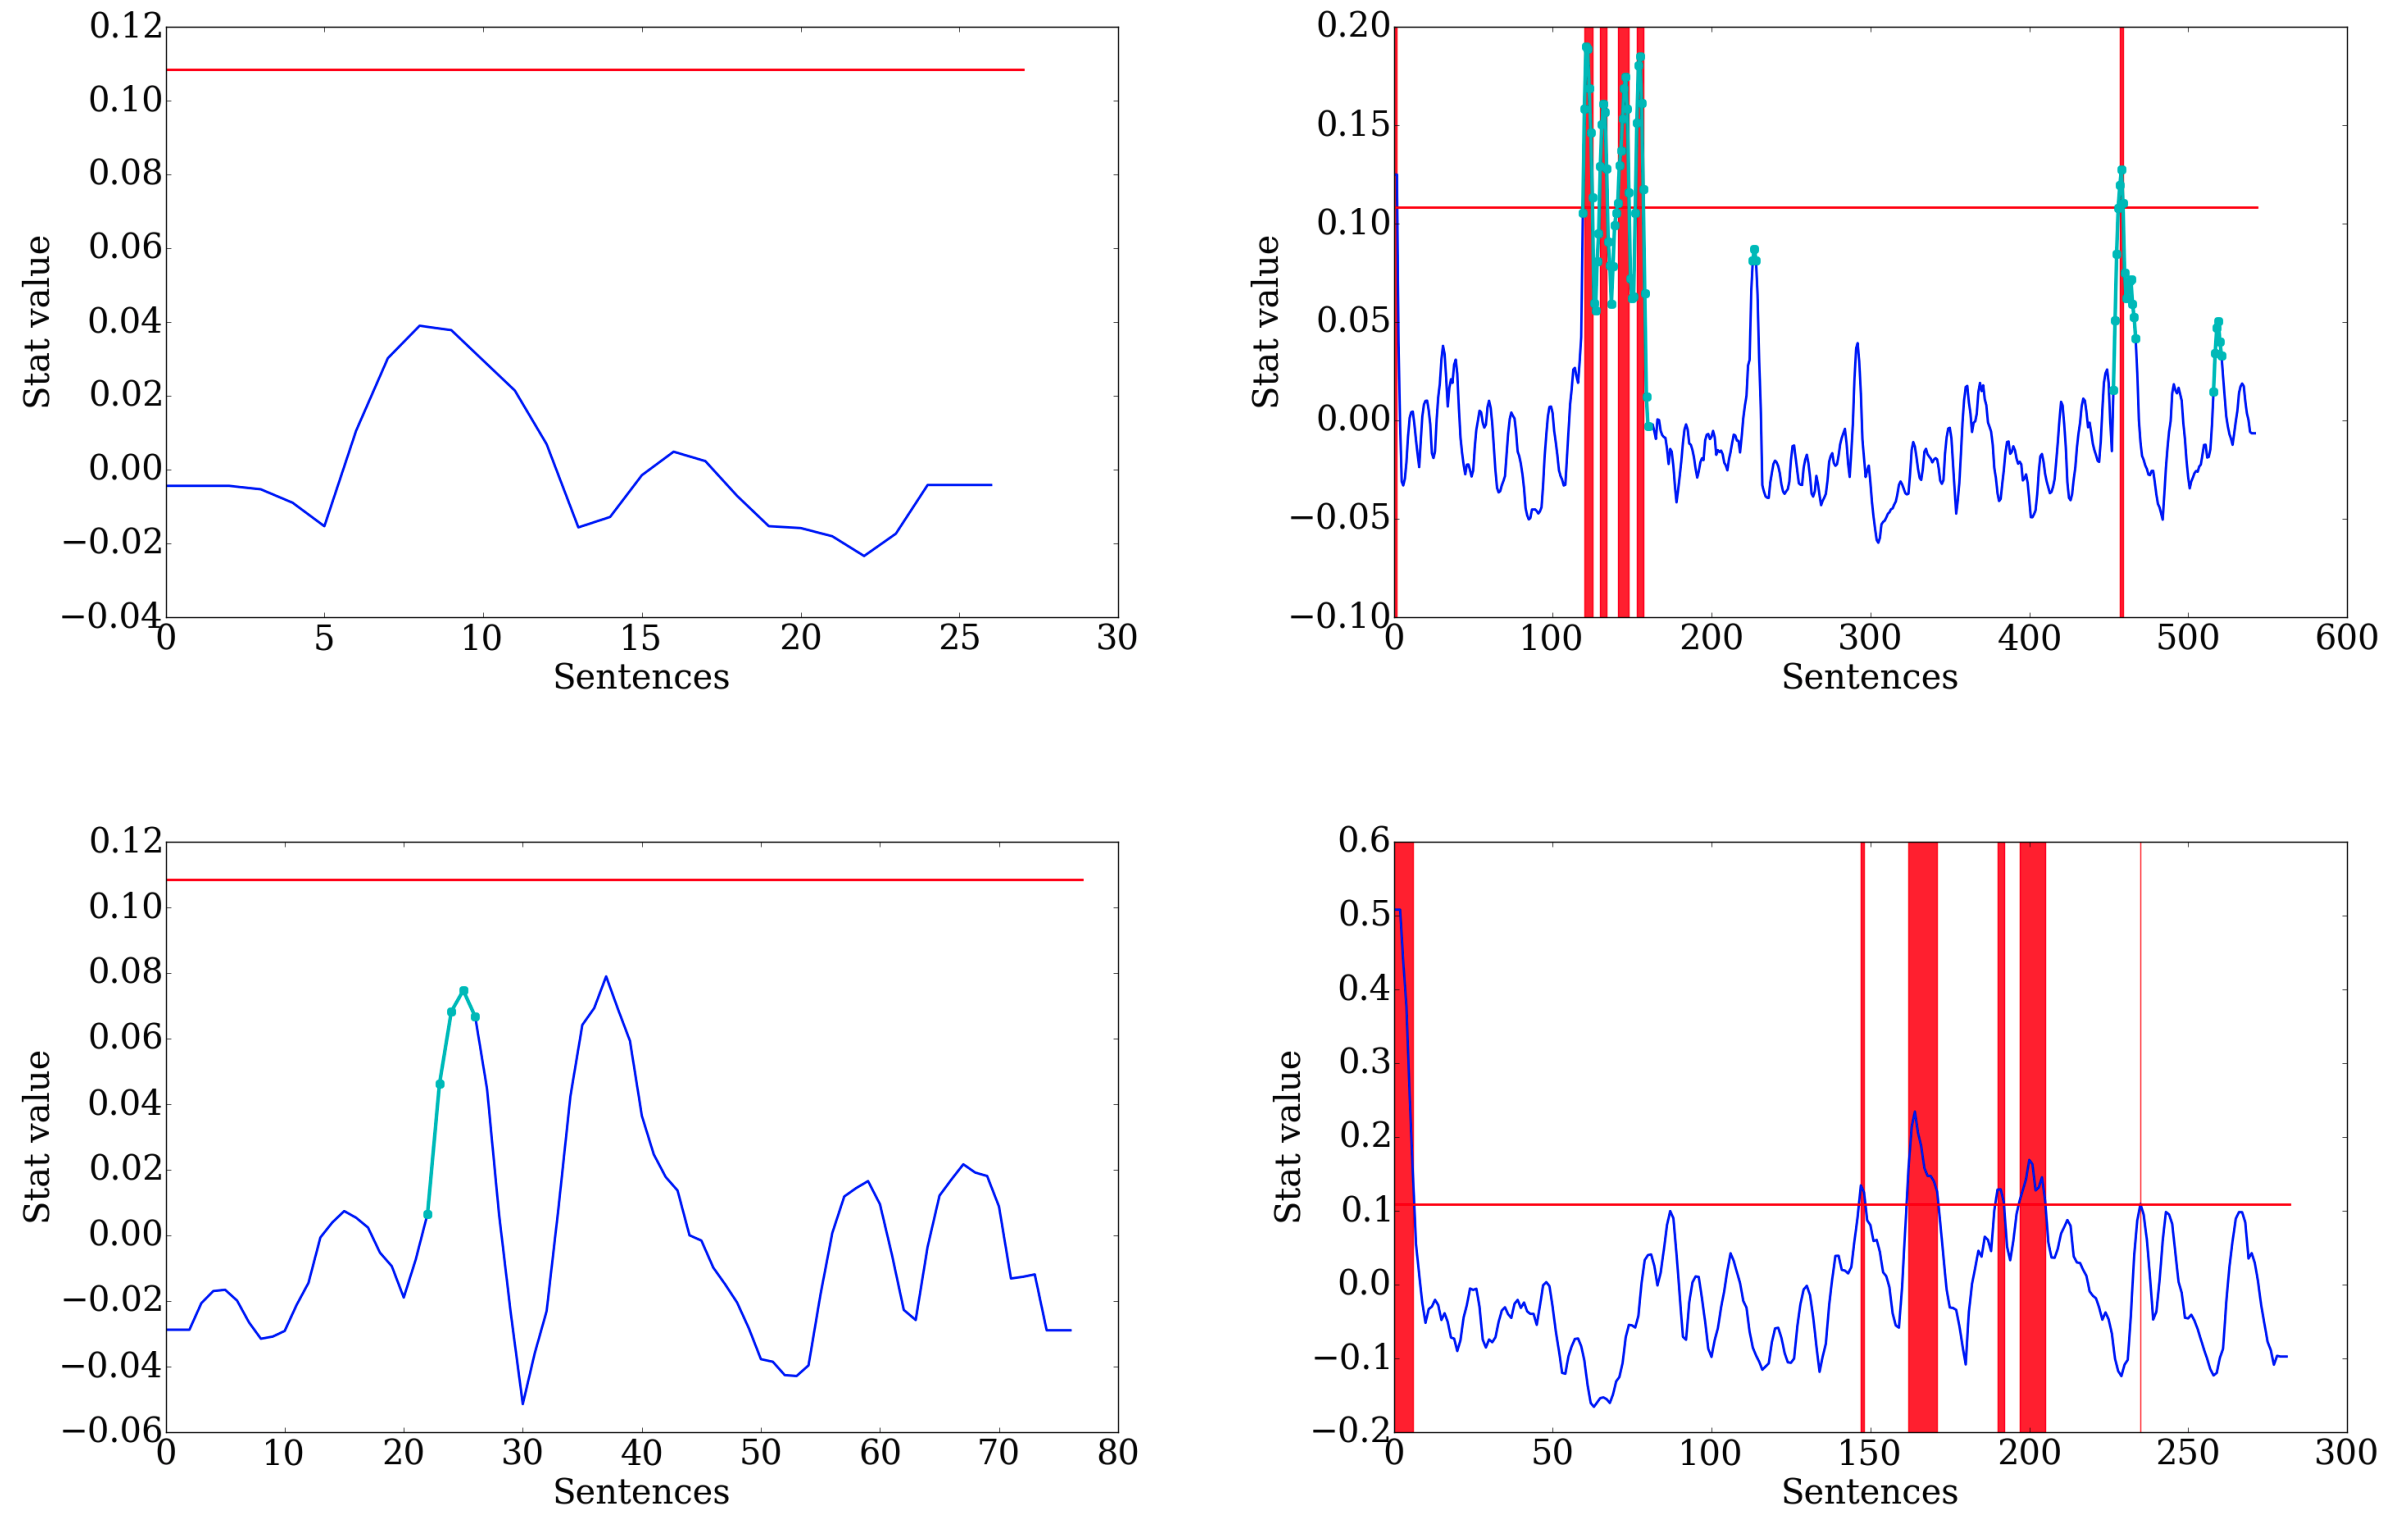
\includegraphics[scale=.26]{clef_text_as_time_series}\\
\centering{Plagiarism detection examples}

\end{frame}
%=============================================
\begin{frame}{Appendix: text data as time series, illustration (2)}

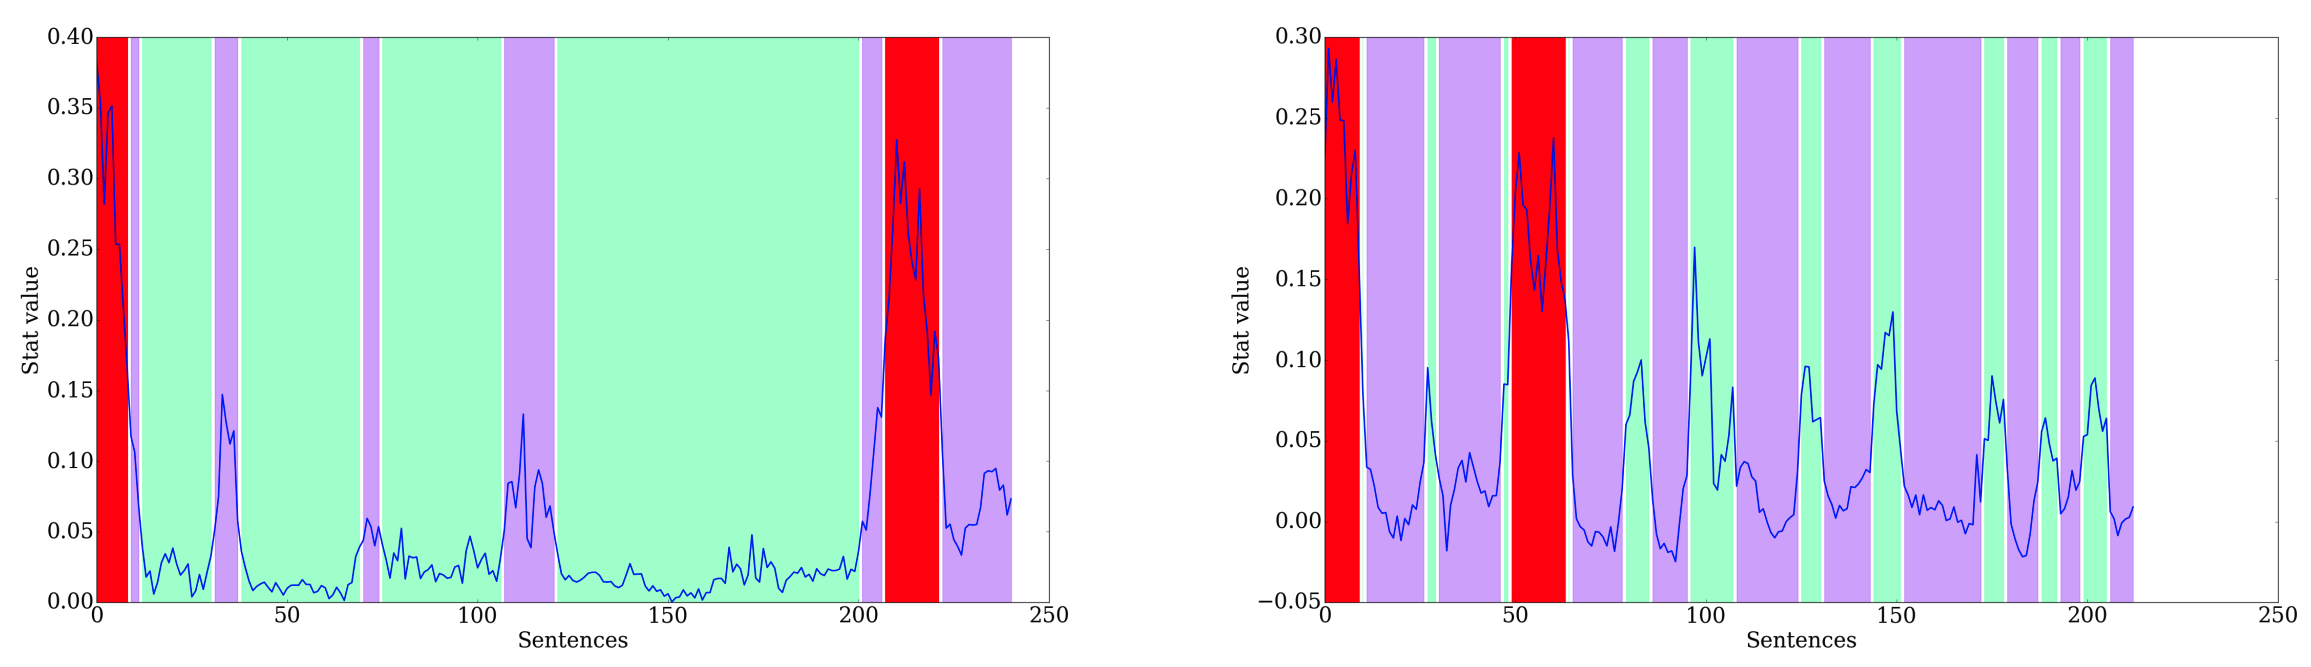
\includegraphics[scale=.27]{clef_text_segmentation}\\
\centering{Text segmentation markdown}

\end{frame}
%=============================================
\begin{frame}{Appendix: phase trajectory of time series}

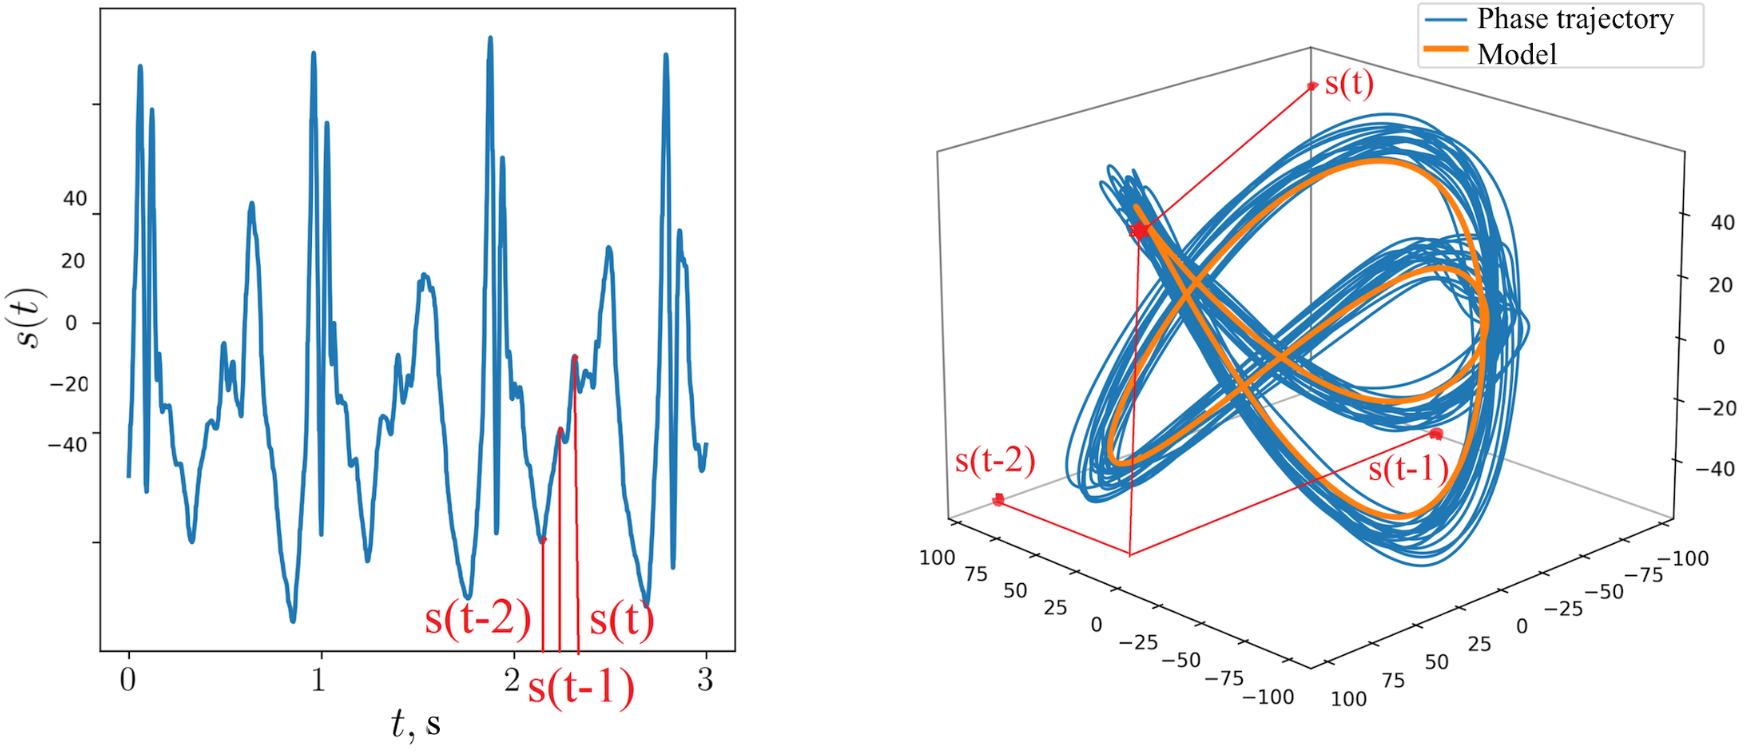
\includegraphics[scale=.37]{phase_trajectory_dimensionality}\\
\centering{Delay embedding delivers dimensionality reduction and keeps the reconstruction}

\end{frame}
%=============================================
\begin{frame}{Appendix: convergent cross-mapping}

{\centering{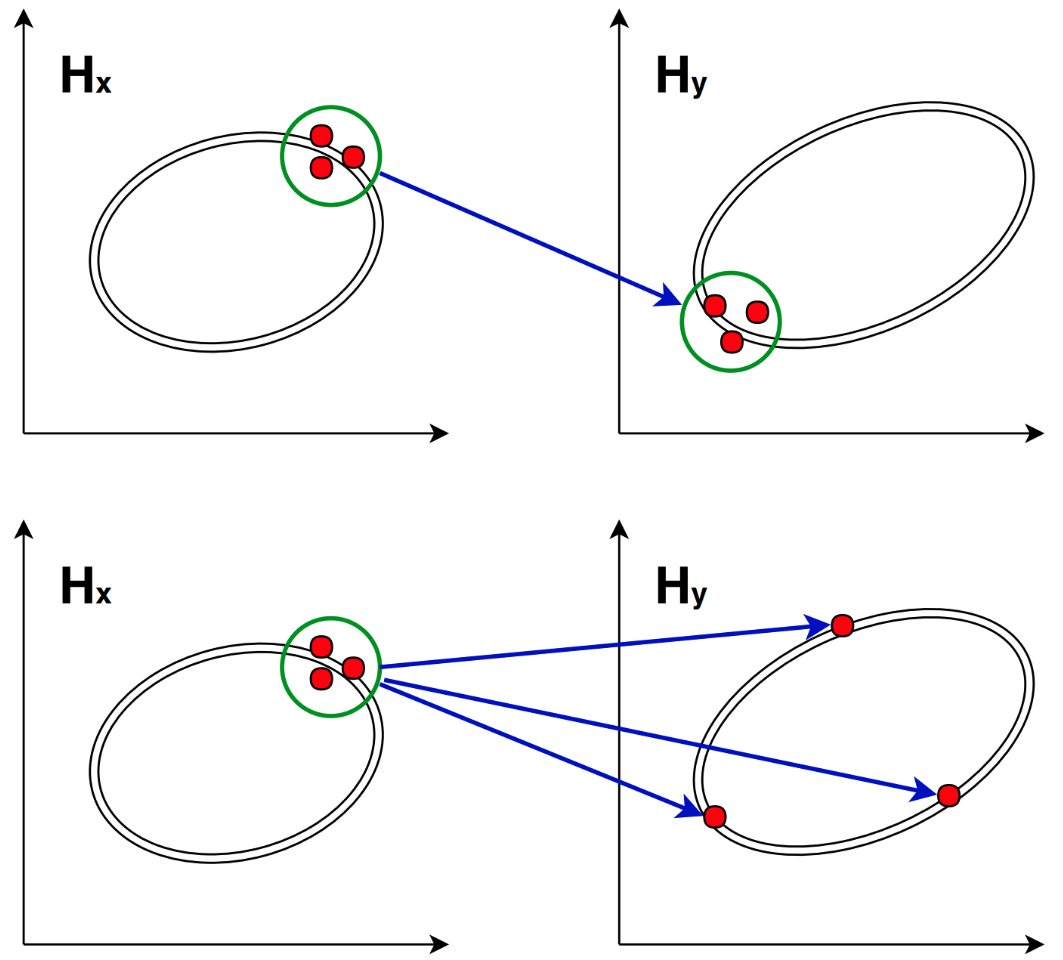
\includegraphics[scale=.35]{convergent_cross-mapping}}\\
\centering{The time series $y$ depends on the time series $x$, but not vice versus}}\\

\bigskip
The time series $y$ depends on the time series $x$, if in the
neighbourhood $(x,x^\prime) \in H_x$ there exists a \emph{Lipschitz continuous map}
$\varphi H_x \to H_y$  such that  $\rho\bigl(H_y (\varphi(x,x^\prime)\bigr) \geqslant L \rho H_x (x,x^\prime)$.

\end{frame}






The following hypothesis apply for each set:
1. The system state is reconstructable, so there is a pair P,Q and Err for both
2. There is a noise is independent between two sets
3. Variant 1 there is a common basis
4. Variant 2 we need alignment with
5. There is a basis in both spaces and there is a dependency as a
6. bipartite graph
7. triangular graph





%=============================================
\end{document}

\begin{frame}{Delay Embedding}

A time series $\{x_i\}_1^N$ is an array of $N$ numbers
\begin{itemize}
    \item representing the values of some measured (observed) dynamical variable $\mathbf{x}(t)$,
    \item taken at a constant time step $\Delta t$.
\end{itemize}

Often, it is convenient to represent a time series in the form of \textit{phase trajectories} — instead of using the variables of the system directly, we use delay vectors:
$$ \mathbf{z}_i = [x_i, x_{i-1}, \dots, x_{i-m+1}]. $$
Each such vector is an element of the $m$-dimensional phase space $\mathbb{R}^m$.
\end{frame}
%=============================================
\begin{frame}{Elements of Takens' Theory}

\begin{itemize}
    \item Let a dynamical system $f(\mathbf{x})$ be given with phase space $\mathbb{R}^M$.
    \item The quantities forming the time series are the values of some function $h$ of the state $\mathbf{x}(t)$ of this dynamical system on a manifold $W^d \subset \mathbb{R}^M$:
    $$ h: W^d \rightarrow \mathbb{R}, \qquad x_i = h(\mathbf{x}(t_i)) = h(f(\mathbf{x}_0, t_i)). $$
    \item With a fixed time step $\Delta t$:  
    $$ \mathbf{x}(t) = f(\mathbf{x}_0, t_i + i \cdot \Delta t). $$
\end{itemize}

Therefore, for the components of the delay vectors we have:

$$ x_i = h(\mathbf{x}(t_i)) = h(f(\mathbf{x}_0,t_i)) $$
$$ x_{i+1} = h(\mathbf{x}(t_{i+1})) = h(f(\mathbf{x}_0, t_i + \Delta t)) $$
$$ \dots $$
$$ x_{i+m-1} = h(\mathbf{x}(t_{i+m-1})) = h(f(\mathbf{x}_0, t_i + (m-1)\cdot \Delta t)) $$

\end{frame}

%=============================================
\begin{frame}{Elements of Takens' Theory}

Since all components of the vector  
$$\mathbf{z}_i = [x_i, x_{i-1}, \dots, x_{i+m-1}]$$  
can be associated with the same measurement of the dynamical system's state  
$$x_i = h(f(\mathbf{x}_0, t_i)),$$  
there exists a vector-valued function $\Lambda$ that maps $x_i$ into vectors in the $m$-dimensional space $\mathbb{R}^m$:

$$
\mathbf{z}_i = \Lambda(x_i), \qquad \mathbf{z}_i \in \mathbb{R}^m.
$$

These considerations form the core of Takens' theorem, which states that when  
$$ m \geq 2d + 1, $$  
the mapping $\Lambda$ constitutes an embedding of the manifold $W^d$ into $\mathbb{R}^m$.

\end{frame}
%=============================================

\end{document}